\documentclass[18pt]{beamer}
%% SLIDE FORMAT
\usepackage[utf8]{inputenc}
\usepackage{algpseudocode}



\title[Programmieren Tutorium]{6. Programmieren Tutorium:\texorpdfstring{\\}{} Objektorientierungs}
\subtitle{Fancy Stuff}
\author{Konstantin Zangerle \texorpdfstring{\\}{} info@konstantinzangerle.de}
\date{7. Dez 2015}

\usepackage{listings}
\usepackage{color}

\definecolor{mygreen}{rgb}{0,0.6,0}
\definecolor{mygray}{rgb}{0.5,0.5,0.5}
\definecolor{mymauve}{rgb}{0.58,0,0.82}

\lstset{ %
  backgroundcolor=\color{white},   % choose the background color
  basicstyle=\footnotesize,        % size of fonts used for the code
  breaklines=true,                 % automatic line breaking only at whitespace
  captionpos=b,                    % sets the caption-position to bottom
  commentstyle=\color{mygreen},    % comment style
  escapeinside={\%*}{*)},          % if you want to add LaTeX within your code
  keywordstyle=\color{blue},       % keyword style
  stringstyle=\color{mymauve},     % string literal style
  showstringspaces=false,
  language=Java
}
\beamersetuncovermixins{\opaqueness<1>{0}}{\opaqueness<2->{0}} %Dont show things after pause 
% Bibliography

\begin{document}

% change the following line to "ngerman" for German style date and logos
%\selectlanguage{ngerman}

%title page
\begin{frame}
\titlepage
\end{frame}

%table of contents
\begin{frame}{Gliederung}
\tableofcontents
\end{frame}

\section{Organsiatorisches}

\begin{frame}{Weihnachten}
 \begin{itemize}
  \item Tutorien bis 22.12
  \item VL am 23.12 fällt aus
  \item 4. Blatt am 9.12 13:00 Ausgabe
  \item Ende 4. Blatt 23.12 13:00
  \item Tuts wieder ab dem 13.1.2016
  \item Dieses Tut also ab dem 18.1.2016
 \end{itemize}

\end{frame}



\begin{frame}{Konstruktoren und super}
 \begin{alertblock}{Ein wichtiger Unterschied}
  In Konstruktoren muss der super() Konstruktor als erstes aufgerufen werden,
  oder gar nicht!
 \end{alertblock}
\end{frame}


\begin{frame}[fragile]{Generische Klassen}
 \begin{lstlisting}
  ArrayList<String> liste = new ArrayList<String>(); //oder...
  Liste liste = new ArrayList<String>();
 \end{lstlisting}
\end{frame}


\begin{frame}[fragile]{Schnittstellen}
\begin{lstlisting}
 interface Motor {
  public void starten();
  public int getLeistung();
 }
 \end{lstlisting}
 \begin{itemize}
  \item Interfaces stellen eine Schablone dar.
  \item Interfaces geben die Gewissheit, das Klassen, die diese implementieren, Funktionen besitzen.
  \item Interfaces haben keine Attribute.
 \end{itemize}

\end{frame}




\end{frame}


\begin{frame}{Queue, Stack, Priority Queue}
\begin{itemize}
 \item Priority Queue \url{http://stackoverflow.com/questions/683041/java-how-do-i-use-a-priorityqueue}
 \item Stack \url{http://www.java-tutorial.org/stack.html}
\end{itemize}

 
\end{frame}

\begin{frame}[fragile]{instanceof}
 \begin{lstlisting}
class Parent {  }
class Child extends Parent {   }

public class Main {
  public static void main(String[] args) {

    Child child = new Child();
    if (child instanceof Parent) {
      System.out.println("passt");
    }

  }

}
 \end{lstlisting}

\end{frame}


%Lacher zum Schluss
\begin{frame}
 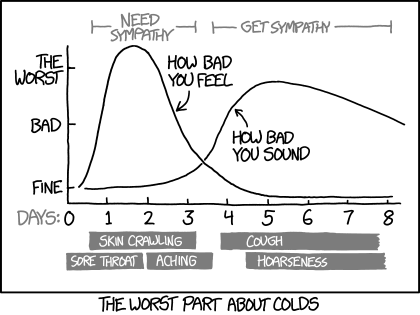
\includegraphics[scale=0.7]{colds}
 
 \tiny{Quelle: xkcd.com/1612}
\end{frame}


\end{document}
%%%%%%%%%%%%%%%%%%%%%%%%%
%Bausteine
%nice to have code
%%%%%%%%%%%%%%%%%%%%%%%%%%



%%%%% Bausteine Folie mit Java-Code
%\begin{frame}[fragile]{bla}
%\begin{exampleblock}{bla}
%\begin{lstlisting}[language=java]
%\end{lstlisting}
%\end{exampleblock}
%\end{frame}
